\chapter{Vision-based Multi-Agent Autonomous Docking Using a Deep Spiking Neural Network and Reward-modulated Spike-Timing-Dependent Plasticity}

\section{Preliminaries}
\subsection{Problem definition: Docking Missions with Swarm Robots}

Swarm robotics, inspired by the collective behaviors observed in natural systems such as ant colonies, bee swarms, and flocks of birds, represents a promising paradigm for creating intelligent robotic systems capable of performing complex, decentralized tasks. These systems are typically characterized by a large number of relatively simple robots that collaborate and coordinate their actions without reliance on any form of centralized control. This decentralized approach offers inherent advantages, including robustness to individual robot failures, flexibility in adapting to changing environments, and scalability to large numbers of agents \cite{dias2021swarm}. 


\begin{figure}[H]
    \centering
    \includegraphics[width=0.9\linewidth]{Figures/Figure 1.pdf}
    \caption{Swarm of robots performing docking mission. Each agent pushes the Payload towards the Central Hub to align them together. The central Hub and agents are equipped with a \ac{dvs} that streams high-frequency data for the proximity mission.}
    \label{fig:DockingMissionfigure}
\end{figure}

The desired collective behavior of the swarm emerges from the local interactions among the individual robots and between the robots and their environment. This paradigm contrasts with traditional robotic systems, which often rely on a central controller to dictate the actions of individual robots. The term ``docking missions," within the context of swarm robotics, encompasses a range of cooperative tasks where multiple robots need to achieve a state of connection or close proximity. This includes tasks such as rendezvous, where the objective is for multiple robots to converge at a common location or maintain a defined spatial relationship; assembly, where robots collaboratively work to form a desired structure or connect with other robots or objects to create a larger, functional entity.

In the specific application of this study, the swarm agents are tasked with pushing a payload towards a central hub to achieve a precise docking alignment. Each agent is equipped with thrusters allowing them to move in a 2D space, and a \ac{dvs} mounted onboard provides them with visual feedback about the environment and neighboring agents. Additionally, a \ac{dvs} camera is mounted at the center of the central hub, offering a global event-based view of the payload and the agents during the docking process.

The primary objective of this paper is to develop a decentralized vision-based swarm docking system utilizing Deep \ac{snn}s trained with \ac{stdp}, which leverages the asynchronous, sparse, and high-temporal-resolution output of \ac{dvs} cameras to guide the swarm behavior effectively. Each agent in the swarm runs its own local \ac{snn} onboard, processing sensory information independently and learning control policies in a distributed manner, which allows the swarm to remain scalable and robust to individual agent failures.

In this environment, \ac{alm}s are installed on both the payload and the agents to enable robust object detection and differentiation within the event-based vision system. Each \ac{alm} transmits light at a specified frequency but with unique phase offsets assigned to the payload and each agent. This phase-based encoding ensures that at each detection interval, only one object's \ac{alm} is illuminated, allowing the system to isolate and identify the payload or specific agents without ambiguity in the \ac{dvs} data stream. This structured blinking strategy facilitates clean separation of objects in the spatiotemporal event data, enabling the network to distinguish between the payload and agents during the docking mission while maintaining the asynchronous and high-temporal-resolution advantages of event-based sensing.

When the agents are flying and have not made contact with the payload, they rely solely on their onboard \ac{dvs} for environment perception, capturing events corresponding to nearby agents and the payload. Once an agent makes physical contact with the payload, its onboard force contact sensor activates, and the onboard \ac{dvs} data is replaced by the central hub \ac{dvs}, providing a more comprehensive and centralized perspective of the payload and the surrounding agents.


\subsection{Event-Based Camera Simulation}

This section presents the simulation methodology for modeling brightness-based visual input and generating asynchronous events for \ac{snn}s using \ac{dvs}. Two distinct \ac{dvs} camera models are used in this study: one mounted on each agent and one placed at a fixed position on the central hub. Both cameras independently perceive the environment and produce separate event streams based on the change in perceived brightness over time.

The environment is populated by multiple agents and a payload object, each modeled as circular shapes with defined physical properties such as radius and centroid location. Each \ac{dvs} camera discretizes its field of view into a grid of $N_y \times N_x$ pixels, where each pixel corresponds to a fixed location in the simulated physical space. The spatial mapping between the continuous world coordinates and the discrete \ac{dvs} pixel grid is defined through a static transformation.

For each \ac{dvs} view, a brightness map is generated at every simulation time step. Let $X_w$ and $Y_w$ represent the 2D coordinate meshgrids over the \ac{dvs} image plane in world units. The initial brightness grid $E(x,y)$ is set to a constant background value $I_{\text{bg}}$ across all pixels. The contribution of each object (agent or payload) to the brightness grid is computed by rendering its circular projection into the grid and modulating its intensity based on relative spatial orientation and distance to one or more luminous sources.

Let $(x_o, y_o)$ denote the position of an object with radius $r_o$. For each pixel with world coordinates $(x_w, y_w)$, we first compute the squared Euclidean distance to the object center:
\begin{equation}
d^2 = (x_w - x_o)^2 + (y_w - y_o)^2.
\end{equation}

Pixels satisfying $d^2 \leq r_o^2$ are considered to lie within the object’s projection. For these pixels, brightness is calculated based on Lambertian reflectance with multiple light sources. Let $(x^{(l)}_s, y^{(l)}_s)$ denote the position of the $l$-th light source. We define the vector from the pixel to the light source as:
\begin{equation}
\mathbf{v}_{\text{light}}^{(l)} = 
\begin{bmatrix}
x_w - x^{(l)}_s \\
y_w - y^{(l)}_s
\end{bmatrix}, \qquad
||\mathbf{v}_{\text{light}}^{(l)}|| = \sqrt{(x_w - x^{(l)}_s)^2 + (y_w - y^{(l)}_s)^2}.
\end{equation}

Similarly, the vector from the pixel to the object center is:
\begin{equation}
\mathbf{v}_{\text{center}} = 
\begin{bmatrix}
x_o - x_w \\
y_o - y_w
\end{bmatrix}, \qquad
||\mathbf{v}_{\text{center}}|| = \sqrt{(x_o - x_w)^2 + (y_o - y_w)^2}.
\end{equation}

The angle $\theta^{(l)}$ between these two vectors is used to compute the cosine-based brightness contribution from light source $l$:
\begin{equation}
\theta^{(l)} = \arccos\left(\frac{\mathbf{v}_{\text{light}}^{(l)} \cdot \mathbf{v}_{\text{center}}}{||\mathbf{v}_{\text{light}}^{(l)}|| \cdot ||\mathbf{v}_{\text{center}}|| + \varepsilon}\right),
\end{equation}
\begin{equation}
I^{(l)} = \max\left(0, \cos(\theta^{(l)}) \cdot 0.5 + 0.5\right),
\end{equation}
where $\varepsilon$ is a small constant to avoid division by zero. The final brightness value at each pixel is computed as the maximum contribution across all light sources and overlapping objects:
\begin{equation}
E(x_w, y_w) = \max\left( I_{\text{bg}}, \max_{\text{objects}} \max_l I^{(l)} \right).
\end{equation}

Once the brightness map $E(x,y)$ is generated, it is passed to the event generation module that models the behavior of the \ac{dvs} sensor. To emulate the logarithmic response of biological photoreceptors, the brightness is first clamped to a minimum value and transformed into logarithmic intensity:
\begin{equation}
E_{\text{clamped}}(x,y) = \max(E(x,y), I_{\min}), 
\end{equation}
\begin{equation}
\mathcal{L}_{\text{current}}(x,y) = \ln(E_{\text{clamped}}(x,y)).
\end{equation}

The temporal contrast is computed as the difference between the current and previously stored logarithmic intensity:
\begin{equation}
\Delta \mathcal{L}(x,y) = \mathcal{L}_{\text{current}}(x,y) - \mathcal{L}_{\text{prev}}(x,y).
\end{equation}

This change in intensity is integrated into a membrane potential variable $V(x,y)$ for each pixel:
\begin{equation}
V_t(x,y) = V_{t-1}(x,y) + \Delta \mathcal{L}(x,y),
\end{equation}
subject to optional clipping to prevent numerical instability.

The \ac{dvs} event generation rule triggers ON and OFF events based on threshold crossing behavior. Define thresholds $\vartheta_{\text{on}} > 0$ and $\vartheta_{\text{off}} > 0$. For each pixel, if:
\begin{equation}
\left\{
\begin{aligned}
&\text{if } V(x,y) \geq \vartheta_{\text{on}}: 
&& e(x,y) = +1, 
&& V(x,y) \leftarrow V(x,y) - \vartheta_{\text{on}}, \\
&\text{if } V(x,y) \leq -\vartheta_{\text{off}}: 
&& e(x,y) = -1, 
&& V(x,y) \leftarrow V(x,y) + \vartheta_{\text{off}}.
\end{aligned}
\right.
\end{equation}

Otherwise, no event is generated and $e(x,y) = 0$. These updates are performed for both agent-mounted and hub-mounted \ac{dvs} views independently, using their respective brightness maps and potential histories. The $\mathcal{L}_{\text{current}}$ map is stored as $\mathcal{L}_{\text{prev}}$ for the next time step.

This detailed simulation allows each agent to perceive a localized view of the environment while the central hub maintains a global perspective. 


% Read these papers:
% \begin{itemize}
%     \item Autonomous in-orbit satellite assembly from a modular heterogeneous swarm
%     \item Robust event-triggered game-based attitude control for on-orbit assembly
%     \item Centralized visual-based navigation and control of a swarm of satellites for on-orbit servicing
%     \item Federated Multi-Agent Mapping for Planetary Exploration
% \end{itemize}


\subsection{Dynamic Model of the Payload and Agents}
\label{sec:agent_dynamics}

Each agent in the swarm is modeled as a point mass of mass \( m \) and radius \( \mathcal{R} \). The dynamic state of each agent includes its position, velocity, thrust-based control forces, and interaction forces arising from collisions with other agents and the payload. Additionally, a central payload object with its own dynamics is influenced by contacts with the agents.

The state of agent \( i \) at time \( t \) is defined as $\mathbf{p}_i(t) = \begin{bmatrix} X_i(t) \\ Y_i(t) \end{bmatrix}$ and $\mathbf{v}_i(t) = \begin{bmatrix} V_{x_i}(t) \\ V_{y_i}(t) \end{bmatrix}$, and the control thrusts along the X and Y axes are derived from spike activity in the output layer of a \ac{snn}. Agents and the payload may collide with each other, and these interactions are modeled using a spring-damper system. Let object \( a \) with position \( \mathbf{p}_a \), velocity \( \mathbf{v}_a \), and radius \( R_a \) interact with object \( b \) with position \( \mathbf{p}_b \), velocity \( \mathbf{v}_b \), and radius \( R_b \). The collision force between objects \( a \) and \( b \) is computed as:

\begin{align}
    \delta_{ab} &= R_a + R_b - \|\mathbf{p}_a - \mathbf{p}_b\|, \\
    \mathbf{n}_{ab} &= \frac{\mathbf{p}_a - \mathbf{p}_b}{\|\mathbf{p}_a - \mathbf{p}_b\|}, \\
    \mathbf{v}_{ab}^{rel} &= \mathbf{v}_a - \mathbf{v}_b, \\
    \mathbf{F}_{ab}^{\text{coll}} &= k \cdot \delta_{ab} \cdot \mathbf{n}_{ab} + c \cdot (\mathbf{v}_{ab}^{rel} \cdot \mathbf{n}_{ab}) \cdot \mathbf{n}_{ab},
\end{align}

\noindent where \( k \) and \( c \) are the spring and damping coefficients, respectively. The collision force \( \mathbf{F}_{ab}^{\text{coll}} \) is applied to object \( a \) while an equal and opposite force \( -\mathbf{F}_{ab}^{\text{coll}} \) is applied to object \( b \). This unified formulation applies to all pairwise interactions within the system, including agent-agent and agent-payload collisions, enabling consistent force computation across the entire environment.


The total force applied to each object \( a \) in the system, which can represent either an agent or the payload, is defined as the sum of all interaction forces from other objects and the control thrust applied to the object. The total force is given by:

\begin{equation}
    \mathbf{F}_a^{\text{total}}(t) = -\mathbf{F}_a^{\text{thrust}}(t) + \sum_{b \neq a} \mathbf{F}_{ab}^{\text{coll}}(t),
\end{equation}

\noindent where \( \mathbf{F}_a^{\text{thrust}}(t) \) denotes the applied control thrust on object \( a \) generated by the \ac{snn}. The continuous-time motion of each object \( a \) is then governed by Newton's second law:

\begin{equation}
    \frac{d^2 \mathbf{p}_a(t)}{dt^2} = \frac{\mathbf{F}_a^{\text{total}}(t)}{m_a},
\end{equation}

\noindent where \( \mathbf{p}_a(t) \) denotes its position at time \( t \).

These equations fully describe the continuous-time dynamics of all agents and the payload within the environment, capturing the adaptive response of each object to control inputs and collision forces with other objects in the system. This unified formulation ensures consistent and scalable multi-object simulation, supporting distributed control and local collision handling across all components in the environment.



\subsection{Neuron model}

Biologically inspired spiking neuron models often exhibit rich dynamical behaviors such as excitability, bursting, and bistability. The well-known Izhikevich model \cite{izhikevich2003simple} strikes a balance between biophysical realism and computational efficiency, using only two ordinary differential equations plus a reset condition. The standard Izhikevich model is given by
\begin{equation}
\begin{cases}
\displaystyle \frac{dv}{dt} \;=\; 0.04\,v^2 \;+\; 5\,v \;+\; 140 \;-\; u \;+\; I(t), \\[6pt]
\displaystyle \frac{du}{dt} \;=\; a\,\bigl(b\,v \;-\; u\bigr),
\end{cases}
\label{eq:izhikevich}
\end{equation}
with a reset rule:
\begin{equation}
\text{if } v \ge 30\text{ mV, then }
\begin{cases}
v \leftarrow c,\\
u \leftarrow u + d.
\end{cases}
\end{equation}

\noindent where $a$ and $b$ are the neuron parameters, $v$ is the membrane potential (in mV), $u$ is a slow recovery variable, $I(t)$ is the external input current, and $c$ and $d$ define how the system is reset after a spike. Building on the neuron model and initialization strategies described in the Preliminaries, we now present the structured architecture and training scheme for the proposed deep SNN.

\subsubsection{Random Synaptic Weight Initialization}

The initial synaptic weight matrix \(S\in\mathbb R^{N_\mathrm{post}\times N_\mathrm{pre}}\) is created based on the binary connectivity matrix \(\mathcal C\in\{0,1\}^{N_\mathrm{post}\times N_\mathrm{pre}}\). Each element of \(S\) is given by
\begin{equation}
S(i,j)=
\begin{cases}
w_{ij}, & \mathcal C(i,j)=1,\\
0,       & \text{otherwise,}
\end{cases}
\end{equation}

so that non‐existent connections remain zero.

A scalar parameter \(p_{\mathrm{active}}\in(0,1]\) (default value \(0.10\)) sets the fraction of total incoming weight that may be active at each time step.  If \(\mathcal{W}_{\mathrm{in}}\) denotes the maximum input strength for a given postsynaptic neuron, then the threshold on the sum of raw weights is
\begin{equation}
\Theta \;=\;\frac{\mathcal{W}_{\mathrm{in}}}{p_{\mathrm{active}}}.
\end{equation}

The algorithm proceeds layer by layer.  For layer index \(\ell=2,\dots,n_{\mathrm{L}}\), let \(\mathcal P_\ell\) be the set of postsynaptic neuron indices in layer \(\ell\) and \(\mathcal Q_{\ell-1}\) the set of presynaptic indices in the previous layer. To generate a spatially smooth random gradient over the presynaptic population, the \(N=|\mathcal Q_{\ell-1}|\) presynaptic indices are embedded onto a two‐dimensional grid of size \(\sqrt {N} \times \sqrt N\), and the grid coordinates are
\begin{equation}
\{(x_k,y_k)\}_{k=1}^N\subset\{1,\dots,\sqrt N\}^2.
\end{equation}
A random center
\begin{equation}
\boldsymbol{\mu}
=\Bigl(\tfrac{\sqrt N+1}2,\tfrac{\sqrt N+1}2\Bigr)
+\delta,\quad
\delta\sim\mathcal U\bigl([-0.5\,\sqrt N,\,0.5\,\sqrt N]^2\bigr),
\end{equation}
and width \(\sigma=\sqrt N/3\) define a Gaussian kernel with additive uniform noise:
\begin{equation}
g_k
=\exp\!\Bigl(-\tfrac{(x_k-\mu_x)^2+(y_k-\mu_y)^2}{2\sigma^2}\Bigr)
+\eta_k,\quad
\eta_k\sim\mathcal U([-0.5,\,0.5]).
\end{equation}
Normalizing \(g_k\) by its maximum,
\begin{equation}
\overline{g}_k
=\frac{g_k}{\max \{g_k\}},
\end{equation}
yields values in \([0,1]\).  These are then mapped into the allowed weight range by
\begin{equation}
w_k
= W_{\min} + (W_{\max}-W_{\min})\,\overline{g}_k.
\end{equation}

For each postsynaptic neuron \(i\in\mathcal P_\ell\), let \(\mathcal I_i\subset\{1,\dots,N\}\) be the indices of grid points corresponding to nonzero connections.  The raw incoming weights are \(\{w_j\}_{j\in\mathcal I_i}\).  If their sum exceeds the threshold \(\Theta\), they are uniformly rescaled:
\begin{equation}
\text{if }\sum_{j\in\mathcal I_i}w_j>\Theta,\quad
w_j\;\leftarrow\;
w_j\,\frac{\Theta}{\sum_{k\in\mathcal I_i}w_k},
\quad j\in\mathcal I_i.
\end{equation}

Finally, these weights are placed into the initialization matrix by
\begin{equation}
S\bigl(i,\mathcal Q_{\ell-1}[j]\bigr)
= w_j,
\quad j\in\mathcal I_i,
\end{equation}
ensuring that each neuron’s incoming synaptic strengths obey both the spatial gradient structure and the total‐input constraint.


\subsubsection*{Analytic Determination of Inhibitory Synaptic Weight}

We consider a Class 1 Izhikevich neuron receiving an excitatory drive \(I_{\rm exc}(t)\) and a fixed inhibitory pulse \(I_{\rm inh}(t)\). Spiking ceases when the \(v\)-nullcline in \eqref{eq:izhikevich}
\begin{equation}
0.04\,v^2 + 5v + 140 - u + I = 0
\end{equation}
collides with its extremum, i.e.\ when
\begin{equation}
\frac{\partial}{\partial v}\bigl(0.04\,v^2 +5v +140 -u +I\bigr)=0
\;\Longrightarrow\;0.08\,v + 5 = 0.
\end{equation}
Thus
\begin{equation}
v^* = -\frac{5}{0.08} = -62.5,\quad
u^* = b\,v^*.
\end{equation}
Substituting back, the total critical current \(I_{\rm crit}\) satisfies
\begin{equation}
0.04\,(v^*)^2 + 5\,v^* + 140 - u^* + I_{\rm crit} = 0
\quad\Longrightarrow\quad
I_{\rm crit}
= u^* \;-\;0.04\,(v^*)^2 \;-\;5\,v^* \;-\;140.
\label{eq:Icrit}
\end{equation}

For the canonical Class 1 choice 
\(\;a=0.02,\;b=-0.1,\;c=-55,\;d=6,\) one finds
\begin{equation}
v^*=-62.5,\quad u^*=b\,v^*=6.25,
\end{equation}
\begin{equation}
0.04\,(v^*)^2=156.25,\quad 5\,v^*=-312.5,
\end{equation}
\begin{equation}
I_{\rm crit}
=6.25 -156.25 +312.5 -140 = 22.5.
\end{equation}
Because each spike increments \(u\) by \(d\), the inhibitory weight must compensate for both \(I_{\rm crit}\) and this adaptation.  Therefore we choose
\begin{equation}
w_{\rm inh} \;=\; I_{\rm crit} + d \;=\; 22.5 + 6 = 28.5,
\end{equation}
so that an inhibitory pulse of amplitude \(-\,28.5\) silences the neuron.  Empirically, we confirmed that \(w_{\rm inh}=-28.5\) immediately vetoes spiking and allows rapid recovery when released.

\section{Proposed Neuromorphic Framework}

\subsection{Deep \ac{snn} Structure}

The neural network implemented in this study consists of four layers: an input layer that processes sensory information from a \ac{dvs}, the first hidden layer that learns the visual perception, the second hidden layer that manages the mission phases and separates the policies for formation flying and docking phase, and an output layer responsible for generating control signals to actuate the motors. Each of these layers employs a distinct parameterization of the Izhikevich neuron model to achieve its respective function within the network.

\begin{figure}[H]
    \centering
    \includegraphics[width=0.95\linewidth]{Figures/Deep SNN.pdf}
    \caption{Deep \ac{snn} Architecture with Entropy-Based Adaptive Pooling and Structured Hidden Layers for Swarm Robotics. The purple connections are excitatory, and the yellow connections are inhibitory. }
    \label{fig:deepSNN}
\end{figure}

In this study, we design a deep \ac{snn} architecture tailored for swarm robotics applications requiring real-time perception, decision-making, and control under strict energy and computational constraints. The network architecture comprises an input layer, two structured hidden layers, and an output layer, each utilizing Izhikevich neuron models to capture biologically realistic spiking dynamics while maintaining computational efficiency. The input layer, containing bistable neurons, processes high-frequency event-based data from \ac{dvs}, maintaining stimulus-relevant activity patterns over time. The two hidden layers are structured to facilitate mission-phase switching and context-aware policy learning, with the first hidden layer incorporating \ac{alm} neurons to create an inhibition mechanism for payload-agent channel separation, while the second layer integrates \ac{mps} and \ac{mpc} neurons for phase-gated control and stability during mission transitions. Finally, the output layer, consisting of four spiking neurons, generates directional control signals in the \(x\) and \(y\) axes, enabling adaptive motor control based on the learned spiking activity patterns. 

This architecture supports distributed onboard training using \ac{stdp}, allowing each agent to learn effective control policies directly from event-based sensory input in a scalable and robust manner.

\subsubsection{Input Layer}

The input layer of the proposed \ac{snn} receives event-based visual input from a \ac{dvs}, which generates sparse spatiotemporal signals represented as discrete events: \(+1\) for ON events (increase in brightness), \(-1\) for OFF events (decrease in brightness), and \(0\) for no activity. Let \( X \in \{-1, 0, +1\}^{n \times n} \) denote the event matrix at a given time step or after temporal accumulation. Due to the high resolution and sparsity of \ac{dvs} data, an adaptive spatial reduction mechanism is applied prior to encoding into spiking neurons.

\paragraph{Entropy-Based Adaptive Pooling}

To reduce dimensionality while preserving information-rich regions, we implement an entropy-guided pooling method. The matrix \( X \) is partitioned into regions \(\Omega\), each corresponding to a pixel in the downsampled output. For a region \(\Omega\), we compute the frequency of event categories:

\begin{equation}
P(c) = \frac{1}{|\Omega|} \sum_{(i,j) \in \Omega} \mathbb{I}(X_{i,j} = c), \quad \text{for } c \in \{-1, 0, +1\}.
\end{equation}

\noindent where, \(\mathbb{I}\) is the indicator function. The Shannon entropy of region \(\Omega\) is then calculated as:

\begin{equation}
H(\Omega) = -\sum_{c \in \{-1, 0, +1\}} P(c) \log_2 P(c),
\end{equation}

\noindent excluding terms where \( P(c) = 0 \). This entropy quantifies the diversity of event types in the region, with \( H(\Omega) = 0 \) indicating uniform activity and \( H_{\max} = \log_2(3) \approx 1.585 \) indicating maximum variability.

The entropy value is then mapped to a pooling kernel size \( k \in [k_{\min}, k_{\max}] \), using a linear transformation:

\begin{equation}
k(H) = k_{\max} - (k_{\max} - k_{\min}) \cdot \frac{H(\Omega)}{H_{\max}}.
\end{equation}

Low-entropy (homogeneous) regions are pooled using a larger kernel \( k_{\max} \), while high-entropy (heterogeneous) regions are pooled more finely. For each subregion, we apply sign-preserving max pooling by selecting the element with the highest absolute value. The resulting values form a downsampled matrix \( X' \in \{-1, 0, +1\}^{n' \times n'} \), where \( n' < n \).

\paragraph{Current Encoding and Input Neuron Configuration}

Each element \( X'_{i,j} \) in the pooled matrix is mapped to an input current \( I_{i,j} \) via a transformation function \( \Gamma(\cdot) \):

\begin{equation}
I_{i,j} = \Gamma(X'_{i,j}),
\end{equation}
where \( \Gamma \) maps the discrete event values into continuous current levels suitable for the neuron model. For example, ON events may produce a positive input current, OFF events a negative current, and silent regions yield no current. The input layer consists of Bistable spiking neurons, each implemented using the Izhikevich neuron model operating in the bistable regime. This configuration allows neurons to remain in a stable spiking or resting state, enabling persistent memory of recent inputs. At steady state, setting \( dv/dt = du/dt = 0 \) in the Izhikevich model leads to the following fixed-point equations:

\begin{align}
u &= bv, \\
0.04v^2 + (5 - b)v + (140 + I) &= 0.
\end{align}


The solutions \( v^* \) to the quadratic equation represent the possible membrane potentials at which the neuron may remain at equilibrium. The number and nature of these solutions depend on the discriminant of the quadratic:
\begin{equation}
\Delta = (5 - b)^2 - 4 \cdot 0.04 \cdot (140 + I).
\end{equation}

When \( \Delta > 0 \), there are two distinct real roots, indicating the existence of two equilibrium points. If one of these is a stable resting state and the other is associated with an unstable point surrounded by a stable limit cycle, the neuron exhibits bistability. This means it can remain in a quiescent (non-spiking) state or transition into repetitive spiking depending on the input and initial conditions.

To examine the local stability of each equilibrium point \( (v^*, u^*) \), the system is linearized using the Jacobian matrix:
\begin{equation}
J(v^*, u^*) =
\begin{pmatrix}
\frac{\partial}{\partial v}(0.04v^2 + 5v + 140 - u + I) & \frac{\partial}{\partial u}(0.04v^2 + 5v + 140 - u + I) \\
\frac{\partial}{\partial v}(a(bv - u)) & \frac{\partial}{\partial u}(a(bv - u))
\end{pmatrix}
=
\begin{pmatrix}
0.08v^* + 5 & -1 \\
ab & -a
\end{pmatrix}.
\end{equation}

The trace and determinant of the Jacobian are given by:

\begin{equation}
\text{Tr}(J) = 0.08v^* + 5 - a = 0.08v^* + 4, \qquad \det(J) = -a(0.08v^* + 5) + ab = -0.08v^* - 3.5.
\end{equation}


The stability of the equilibrium point depends on the sign of these values. If \( \text{Tr}(J) < 0 \) and \( \det(J) > 0 \), then the equilibrium is stable, and if \( \text{Tr}(J) > 0 \) or \( \det(J) < 0 \), then the equilibrium is unstable. Because both trace and determinant depend on the specific value of \( v^* \), it is possible for one root to correspond to a stable resting state (e.g., \( v^* \approx -60 \, \text{mV} \)) while the other leads to an unstable point surrounded by a spiking limit cycle. This configuration underlies the bistable behavior of the neuron, allowing it to encode information persistently across time depending on the strength and polarity of the injected current.


Each neuron receives input from the preprocessed \ac{dvs} event matrix, where ON events (\(+1\)) and OFF events (\(-1\)) are mapped to distinct neuron indices. Neurons corresponding to ON events are injected with maximum excitatory current \( I = 100 \, \text{nA} \), and those corresponding to OFF events receive strong inhibitory input \( I = -80 \, \text{nA} \). All other neurons maintain a baseline current of \( I = -65 \, \text{nA} \), representing a resting or non-stimulated state. This behavior is encoded as:

\begin{align}
I_i(t) =
\begin{cases}
100 \, \text{nA}, & \text{if } X'_{i} = +1, \\
-80 \, \text{nA}, & \text{if } X'_{i} = -1, \\
-65 \, \text{nA}, & \text{otherwise}.
\end{cases}
\end{align}

This input mapping is crucial in shaping the dynamic behavior of bistable neurons. In the case of an ON event, the neuron receives a transient positive input current that is applied for a single simulation step. However, due to the bistable nature of the model, the neuron does not immediately return to rest after the stimulus disappears. Instead, it remains in an active spiking state, continuously firing until it is explicitly reset by an OFF event. This reset occurs when the same neuron index receives an inhibitory current corresponding to a negative event in the \ac{dvs} stream.

This mechanism enables the input layer to function as a short-term memory system. Even in the absence of new motion or visual changes in the environment, neurons that were previously excited by object movement continue to spike, thereby maintaining a persistent representation of object locations. As a result, the network retains awareness of the last known positions of salient features, making it especially suitable for processing sparse, asynchronous data and tracking static or intermittently visible targets.

\subsubsection{Hidden Layers}
\subsubsection*{First Hidden Layer for Visual Processing of \ac{dvs} Events}

The first hidden layer of the \ac{snn} is designed to perform early-stage visual feature extraction, dimensionality reduction, and fuzzy separation of the environment while incorporating \ac{alm}-based attention and gating mechanisms. This layer contains three repositories of neurons that collectively process the preprocessed \ac{dvs} input to distinguish between the payload and neighboring agents while encoding these features in a fuzzy spatial representation.

\begin{figure}[H]
    \centering
    \includegraphics[width=1\linewidth]{Figures/Hidden Layer 1.pdf}
    \caption{Structured First Hidden Layer Architecture with \ac{alm}, Payload, and Agent Perception Repositories for Visual Perception.}
    \label{firsthiddenlayer}
\end{figure}

All neurons in this layer utilize the Izhikevich neuron model configured for Class 1 excitability, enabling the neurons to modulate their spiking frequency smoothly in response to the strength of the injected input currents. To implement \ac{alm}-based attention, the \ac{alm} neurons in the layer are configured for tonic bursting to ensure persistent spiking during activation windows. For these neurons, the same initialization of the membrane potential and recovery variables ensures consistent readiness for event-driven activation.

The \ac{alm}s are mounted on the payload, and each agent transmits light periodically at a frequency designed for phase-shifted activation patterns. The payload's \ac{alm} is configured to blink with a period \( T_P = 20 \, \text{ms} \), remaining active for \( T_{P}^{\text{on}} = 10 \, \text{ms} \) with a phase offset of \( \phi_P = 0 \, \text{ms} \). Each agent's \ac{alm} operates with the same period and activation duration but with a phase offset of \( \phi_A = 10 \, \text{ms} \) relative to the payload, ensuring that the agents' \ac{alm}s are active precisely when the payload's \ac{alm} is inactive. This relationship can be expressed as:

\[
\text{Active}_{\text{ALM}}(t) =
\begin{cases}
1, & \text{if } \langle (t - \phi, T) \rangle < T^{\text{on}}, \\
0, & \text{otherwise},
\end{cases}
\]
where \(\phi\) denotes the phase offset for either the payload or agent.

Each time the agent's \ac{alm} activates, the \ac{alm} neurons in the first hidden layer receive input currents and fire spikes. To ensure that these neurons maintain activity throughout the \ac{alm}'s active window and beyond, the stimulation provided to the \ac{alm} neurons is randomized within the activation interval, ensuring a distribution of spike timings that prevents synchronous inactivity between time steps. This mechanism supports consistent gating activity, enabling robust attention control within the spiking network.

Functionally, the first hidden layer separates the payload position channel and the neighboring agents' position channel, representing them in a fuzzy spatial format using the spiking activity of its neurons. This fuzzy coding is achieved by mapping the processed \ac{dvs} input onto the neurons while allowing the network to maintain partial activation across spatial regions, enabling smooth transitions between detected object configurations.

Additionally, the first hidden layer performs dimensionality reduction by compressing the high-resolution \ac{dvs} input into a lower-dimensional representation suitable for the subsequent layers while preserving the essential features necessary for object tracking and environmental understanding. This reduction is crucial for the scalability of the network and for enabling efficient computation during online learning and control.

The spiking patterns generated within this layer create unique states in the network, allowing the system to distinguish different object configurations in the environment robustly. During operation, when the agents' \ac{alm}s are active, the corresponding \ac{alm} neurons in the first hidden layer fire and inhibit the payload detection repository. This gating ensures that during the weight update phase of the network, only the connections associated with the agent detection repository are updated. When the agents' \ac{alm}s turn off and the payload's \ac{alm} activates, the payload detection neurons fire, and the connections associated with the payload detection repository are updated in the subsequent weight update phase.

Through this mechanism, the first hidden layer dynamically manages the flow of information based on the phase-synchronized \ac{alm} signals, ensuring clear separation between agent and payload representations, maintaining fuzzy spatial coding, reducing input dimensionality, and creating structured, distinguishable states for downstream processing in the \ac{snn}.



\subsubsection*{Second Hidden Layer for Mission Phase Switching}

The second hidden layer facilitates mission-phase switching and policy learning by leveraging structured neuron repositories that enable the network to autonomously transition between formation flying and docking phases while learning appropriate control policies through spiking activity.

Within this layer, \ac{ffm} neurons, \ac{mps} neurons, \ac{mpc} neurons, and \ac{cdm} neurons are interconnected to enforce phase-gated learning. The \ac{ffm} and \ac{cdm} neurons act as repositories through which synaptic connections to the output layer are routed, enabling phase-specific learning by ensuring that only active pathways during a particular mission phase undergo synaptic plasticity.

\begin{figure}
    \centering
    \includegraphics[width=1\linewidth]{Figures/Hidden Layer 2.pdf}
    \caption{Structured Second Hidden Layer Architecture with Mission-Phase and Regulatory Neuron Repositories.}
    \label{secondhiddenlayer}
\end{figure}

The neurons within this layer employ models capable of producing persistent spiking, bistability, and rapid state transitions required for dynamic mission control. The \ac{ffm} and \ac{cdm} neurons are configured to exhibit tonic spiking behavior to sustain stable outputs during their respective active phases. In contrast, the \ac{mps} neurons exhibit bistable firing patterns, enabling them to maintain persistent activity while providing controlled inhibition during phase transitions. The \ac{mpc} neurons are designed to generate rapid, transient spiking patterns that effectively trigger phase switches by inhibiting the active repositories when mission conditions change.

During \emph{formation flying}, the agent has not contacted the payload, and the \ac{ffm} neurons maintain persistent spiking activity. Let the activity vector of the \ac{ffm} neurons at time $t$ be denoted by
\begin{equation}
\mathbf{s}_{\mathrm{FFM}}(t) \in \{0,1\}^{N_{\mathrm{FFM}}},
\end{equation}
where $N_{\mathrm{FFM}}$ is the number of \ac{ffm} neurons and $s_{\mathrm{FFM},i}(t)=1$ if the $i$-th neuron spikes at time $t$. To ensure continuous gating, the \ac{ffm} neurons receive random excitatory current $I_{\mathrm{rand}}(t)$ to maintain consistent spiking, leading to persistent inhibition of the \ac{cdm} neurons.

The inhibition of \ac{cdm} neurons by \ac{mps} neurons is modeled as
\begin{equation}
W_{ij}^{\mathrm{CDM} \leftarrow \mathrm{RFP}} = -\gamma,
\end{equation}
where $\gamma > 0$, and the resulting inhibitory current is
\begin{equation}
I_j^{\mathrm{inh}}(t) = \sum_{i} W_{ij}^{\mathrm{CDM} \leftarrow \mathrm{RFP}} s_{\mathrm{RFP},i}(t).
\end{equation}

Simultaneously, the \ac{ffm} neurons provide excitatory input to the \ac{mps} neurons to sustain their spiking:
\begin{equation}
W_{ij}^{\mathrm{RFP} \leftarrow \mathrm{FFM}} = \delta,
\end{equation}
where $\delta > 0$, producing the excitatory current
\begin{equation}
I_j^{\mathrm{exc}}(t) = \sum_{i} W_{ij}^{\mathrm{RFP} \leftarrow \mathrm{FFM}} s_{\mathrm{FFM},i}(t).
\end{equation}

During this phase, the active learning pathway extends from the input layer to the visual processing layer, through the \ac{ffm}, to the output layer, where synaptic connections within the \ac{ffm} repository are updated according to the \ac{stdp} rule. Upon payload contact, the \ac{mpc} neurons are activated, signaling the transition to the docking phase. The \ac{mpc} neurons inhibit both \ac{ffm} and \ac{mps} neurons:
\begin{equation}
W_{ij}^{\mathrm{FFM} \leftarrow \mathrm{MPC}} = -\beta, \quad W_{ij}^{\mathrm{RFP} \leftarrow \mathrm{MPC}} = -\beta,
\end{equation}
where $\beta > 0$, and the induced inhibition is
\begin{equation}
I_j^{\mathrm{MPC-inh}}(t) = \sum_{i} W_{ij}^{\mathrm{FFM/RFP} \leftarrow \mathrm{MPC}} s_{\mathrm{MPC},i}(t).
\end{equation}
This inhibition silences \ac{ffm} and \ac{mps} activity, releasing the \ac{cdm} neurons from inhibition and allowing them to fire, thereby enabling the network to transition to the \emph{docking phase}.

During docking, the active learning pathway becomes the input layer to the visual processing layer, to the \ac{cdm}, and continues to the output layer, allowing the network to learn the docking policy explicitly through the active \ac{cdm} connections.

This structure ensures that only the relevant neuron repository (\ac{ffm} or \ac{cdm}) is active during each mission phase, enforcing phase-specific learning while preventing interference between formation flying and docking. This phase-gated connectivity enables energy-efficient, event-driven learning aligned with the sparse nature of \ac{snn}s, providing reliable mission-phase transitions for autonomous docking missions.



\subsubsection{Output Layer and PWM Signal Generation}

The output layer of the \ac{snn} consists of four neurons configured in the Class 1 excitability regime of the Izhikevich model. This configuration enables a smooth transition from resting to spiking states, allowing the neuron to adjust its firing frequency continuously in response to varying input currents. Such behavior is particularly suitable for motor control, where the precise modulation of thrust must reflect the instantaneous demands of the system.

The output layer neurons correspond to the four directional thrust commands: negative X-axis, positive X-axis, negative Y-axis, and positive Y-axis, indexed respectively as \(\{X^-, X^+, Y^-, Y^+\}\). Each neuron integrates input currents received from the upstream hidden layer and produces spike trains at a temporal resolution determined by the simulation step size.

The Class 1 neurons fire at low and adjustable frequencies, ensuring that the output spiking rate accurately reflects the magnitude of the input current. To compute the motor thrust commands, the spiking activity of each output neuron is sampled at the end of the control update window. Let \( \Delta t \) denote the simulation time step, and let \( T \) denote the control update interval. The binary spike state of each output neuron at the latest simulation time within the interval is denoted by:

\begin{equation}
D_i = \text{f}_i[T/\Delta t],
\end{equation}

\noindent where \( \text{f}_i[k] \in \{0,1\} \) indicates whether neuron \( i \) fired a spike at the \( k \)-th time step. This sampling approach effectively interprets the most recent spike activity of each neuron as a pulse-width modulation (PWM) control signal for the corresponding thrust direction.

The net thrust forces along the X and Y axes are computed as the difference between the PWM signals of opposing direction neurons, scaled by the maximum allowable thrust value \( F_{\text{max}} \):

\begin{align}
F_X^{\text{thrust}} &= F_{\text{max}} \cdot (D_{X^+} - D_{X^-}),\\
F_Y^{\text{thrust}} &= F_{\text{max}} \cdot (D_{Y^+} - D_{Y^-})
\end{align}

This formulation ensures that a recent spike in the \( X^+ \) neuron, for example, results in a positive thrust command along the X-axis, while a spike in the \( X^- \) neuron results in a negative thrust command along the same axis. The same logic applies to the Y-axis neurons.

By using the most recent spike event rather than a time-averaged duty cycle, the system achieves high reactivity, allowing the motor commands to change instantly in response to environmental feedback or network decisions. This approach reduces computational overhead while preserving a direct and biologically inspired mapping between spiking activity and control output. Furthermore, the use of differential encoding across opposing neuron pairs ensures that simultaneous contradictory commands cancel each other out, maintaining system stability and ensuring balanced control actions during fast maneuvers and precision positioning tasks.






\subsection{Training Deep \ac{snn} with \ac{stdp}}

\subsubsection{Reward Function for the First Hidden Layer}

The reward function in the \ac{snn} provides structured, layered feedback to guide synaptic plasticity by aligning the network’s fuzzy internal representations with the event-based sensory input, ensuring adaptive online learning. At each reward computation step, the fuzzy representation of the input layer activity is calculated as the time-averaged firing activity:

\begin{equation}
x_i^{\text{input}} = \frac{1}{T} \sum_{t-T}^{t} f_i,
\end{equation}
where \( f_i(\tau) \in \{0,1\} \) is the binary spiking activity of neuron \( i \) at time \( \tau \), and \( T \) is the update window. Collecting these across all input neurons forms the input activity matrix:

\begin{equation}
\textbf{X}_{\text{input}} = [x_1^{\text{input}}, x_2^{\text{input}}, \ldots, x_N^{\text{input}}],
\end{equation}
where each element indicates the fuzzy membership value of the corresponding feature in the input.

Similarly, for the first hidden layer, the payload detector and agent detector repositories compute:

\begin{equation}
x_i^{\text{hid}} = \frac{1}{T} \sum_{t-T}^{t} f_i^{\text{hid}},
\end{equation}
where \( f_i^{\text{hid}}(\tau) \) is the spiking activity of hidden layer neuron \( i \). These form the matrices \(\textbf{X}_{\text{payload}}\) and \(\textbf{X}_{\text{agent}}\), representing the fuzzy spatial activity maps for the payload and agents, respectively. To compute the attention map, the input activity matrix \(\textbf{X}_{\text{input}} \) is compared with the positions represented in the hidden layer using a Gaussian-weighted mapping. For a hidden layer grid cell at \((x_q, y_q)\) and an input position \((x_k, y_k)\), the squared Euclidean distance is:

\begin{equation}
d_{kq}^2 = (x_k - x_q)^2 + (y_k - y_q)^2.
\end{equation}

The attention weight assigned is:

\begin{equation}
w_{kq} = \exp\left( -\frac{d_{kq}^2}{2 s^2} \right),
\end{equation}
where \( s=[0.05, 0.1] \) is a scale parameter controlling the sensitivity. The \emph{modulation signal} \(\alpha_q\), which serves as the learning rate for each hidden layer neuron, is computed directly by comparing the attention-weighted input activity with the current hidden layer activity:

\begin{equation}
\alpha_q = \frac{\sum_k w_{kq} \cdot x_k^{\text{input}}}{\sum_k w_{kq} + \epsilon} - x_q^{\text{hid}}.,
\end{equation}
where \(\epsilon\) ensures numerical stability. This formulation reduces the dimensionality of the input while emphasizing high-activity regions aligned with the \ac{alm} areas and directly provides the per-neuron learning signal. When the hidden layer activity \( x_q^{\text{hid}} \) matches the attention-driven target, the learning rate satisfies \(\alpha_q \rightarrow 0,\), stopping the weight updates for that neuron during the iteration.


The reward for each hidden layer neuron is defined as:

\begin{equation}
r_q^{(1)} = x_q^{\text{hid}} + \epsilon,
\end{equation}
ensuring the neuron remains responsive to reward-based modulation while avoiding numerical instability. Collecting the rewards across all neurons yields the reward vector:

\begin{equation}
\mathbf{r}^{(1)} = [r_1^{(1)}, r_2^{(1)}, \ldots, r_{N}^{(1)}]^T.
\end{equation}

 Figure \ref{fig:PayloadRewardPipeline} shows how the reward function pipeline works for the agent detection process in the first hidden layer. The modulation signal provides the value of \(\alpha_q\) for each neuron, corresponding to each pixel in the representation.

\begin{figure}[H]
    \centering
    \subfigure[Raw \ac{dvs} Events]{
        \includegraphics[width=0.45\linewidth]{Figures/Payload_RawDVS.pdf}
    }
    \hfill
    \subfigure[Attention Fuzzy Map (16x16)]{
        \includegraphics[width=0.45\linewidth]{Figures/Payload_AttentionFuzzyMap.pdf}
    }
    \vfill
    \subfigure[Hidden Layer Activity (16x16)]{
        \includegraphics[width=0.45\linewidth]{Figures/Payload_HiddenLayerActivity.pdf}
    }
    \hfill
    \subfigure[Post-neuron reward (Modulation Signal)]{
        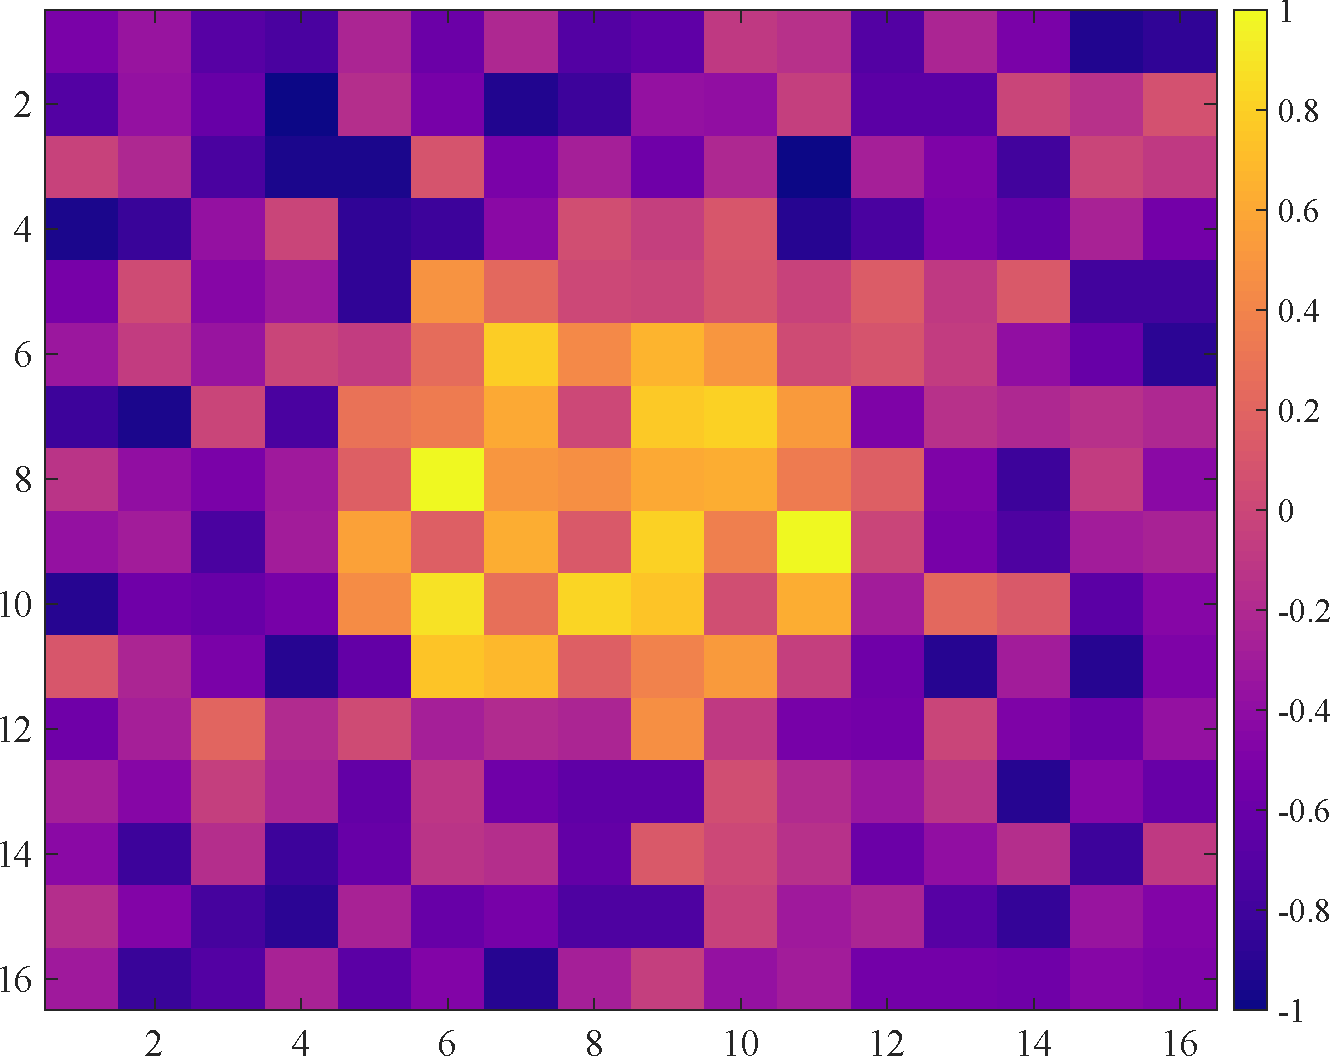
\includegraphics[width=0.45\linewidth]{Figures/Payload_ModulationSignal.pdf}
    }
    \caption{Reward function pipeline for the payload case. The pipeline illustrates the raw \ac{dvs} events, the attention-based fuzzy map, the normalized hidden layer activity during the initial training phase (\(r_q^{(1)}\)), and the modulation signal calculated as the difference between the attention map and the hidden layer activity (\(\alpha_q\)).}
    \label{fig:PayloadRewardPipeline}
\end{figure}


Figure \ref{fig:AgentsRewardPipeline} shows an example of the reward function pipeline for the agent detector repository in the first hidden layer.

\begin{figure}[H]
    \centering
    \subfigure[Raw \ac{dvs} Events]{
        \includegraphics[width=0.45\linewidth]{Figures/Agents_RawDVS.pdf}
    }
    \hfill
    \subfigure[Attention Fuzzy Map (16x16)]{
        \includegraphics[width=0.45\linewidth]{Figures/Agents_AttentionFuzzyMap.pdf}
    }
    \vfill
    \subfigure[Hidden Layer Activity (16x16)]{
        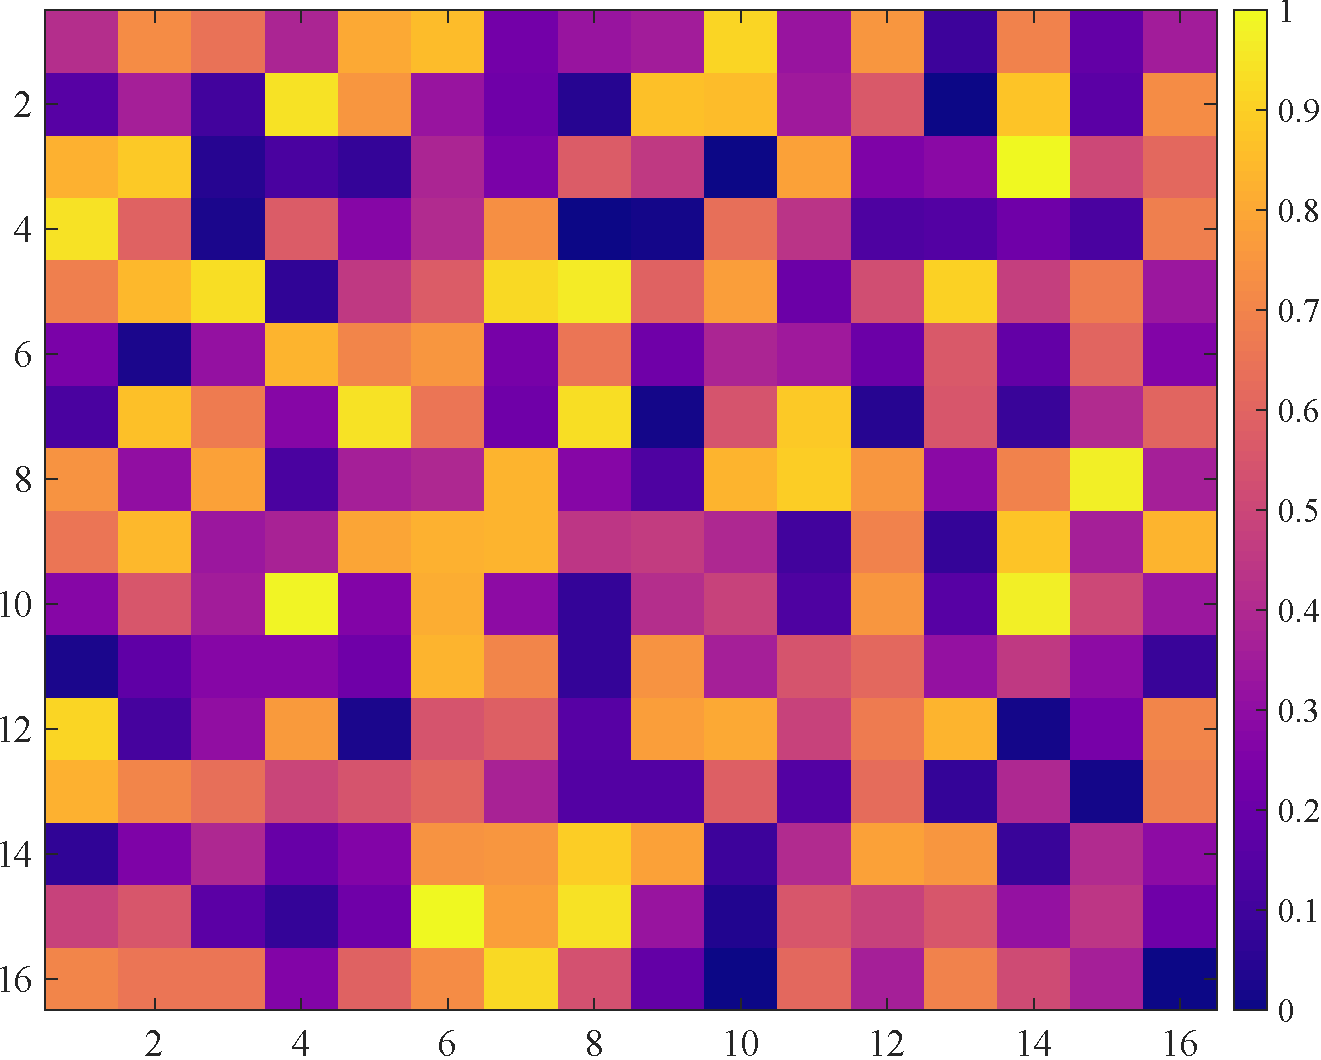
\includegraphics[width=0.45\linewidth]{Figures/Agents_HiddenLayerActivity.pdf}
    }
    \hfill
    \subfigure[Post-neuron reward (Modulation Signal)]{
        \includegraphics[width=0.45\linewidth]{Figures/Agents_ModulationSignal.pdf}
    }
    \caption{Reward function pipeline for the agents case. This pipeline demonstrates the raw \ac{dvs} events for multiple agents, the reduced entropy-based fuzzy map used for attention, the hidden layer’s normalized activity, and the modulation signal computed for reward-based learning in the spiking neural network.}
    \label{fig:AgentsRewardPipeline}
\end{figure}

This design enables the first hidden layer to adaptively learn environmental configurations using event-based, fuzzy attention while regulating learning on a per-neuron basis according to the current match with the input-derived target activity, ensuring efficient, stable convergence in layered \ac{snn} learning.

\subsubsection{Reward Function for the Second and Third Hidden Layers}

For the second hidden layer and the output layer, the reward is computed using a temporally oscillating Gaussian-centered modulation designed to align the network's learning with the spatial focus of the environment, typically the payload during docking and collaborative tasks.

The oscillation frequency is defined by:

\begin{equation}
f_{\text{osc}} = \frac{1}{T_{\text{ALM}}},
\end{equation}
where \( T_{\text{ALM}} \) is the \ac{alm} blinking period of the agent, and the corresponding angular frequency is \(\omega = 2\pi f_{\text{osc}}\) to synchronize the oscillation with the \ac{alm} cycle.

The baseline width of the Gaussian envelope is set to the payload's physical radius \(\sigma_0 = R_P\), and the modulation depth is chosen as \(\alpha = 0.5 \cdot \sigma_0,\) corresponding to 50\% of the baseline width.

Using these parameters, the time-varying width and amplitude of the Gaussian are defined as:

\begin{equation}
\sigma(t) = \sigma_0 + \alpha \cdot \sin(\omega t),
\end{equation}
\begin{equation}
A(t) = \sin(\omega t).
\end{equation}

The oscillating Gaussian envelope over normalized spatial coordinates \((x, y) \in [-1, 1]^2\) is then defined as:

\begin{equation}
G(x, y, t) = A(t) \cdot \exp\left( -\frac{x^2 + y^2}{2 \sigma(t)^2} \right).
\end{equation}

To compute the reward signal, the element-wise product between the normalized sensory event input \( E(x, y) \) and the Gaussian envelope is summed over the grid:

\begin{equation}
\mathcal{R} = \frac{\sum_{x, y} E(x, y) \cdot G(x, y, t)}{\sum_{x, y} |G(x, y, t)| + \epsilon},
\end{equation}
where \( \epsilon \) is a small constant to ensure numerical stability. This scalar reward \(\mathcal{R}\) quantifies how well the sensory input aligns with the oscillating Gaussian focus, dynamically guiding the network to attend to the center of the environment in synchrony with the \ac{alm} cycle.

\begin{figure}[H]
    \centering
    \subfigure[The oscillatory Gaussian envelope when the payload \ac{alm} is active.]{
        \includegraphics[width=0.45\linewidth]{Figures/Payload.pdf}
    }
    \hfill
    \subfigure[The oscillatory Gaussian envelope when the agent \ac{alm} is active.]{
        \includegraphics[width=0.45\linewidth]{Figures/Agent.pdf}
    }
\end{figure}



The computed reward \(\mathcal{R}\) is scaled and uniformly assigned to each neuron in the second hidden layer and the output layer, enabling layered reward-modulated synaptic plasticity in which the second hidden layer and output layer utilize global, oscillation-driven rewards, complementing the fine-grained, per-neuron reward modulation of the first hidden layer. This mechanism ensures the network synchronizes learning with the environment's temporal dynamics while maintaining layered learning efficiency, enabling the \ac{snn} to focus on critical environmental features during operation.

\subsubsection{Weight Update using \ac{stdp}}

During the weight update phase, let \(\mathbf{C}\) denote the submatrix of eligibility traces of synaptic connections from pre-synaptic to post-synaptic neurons in the layer, which changes based on the STDP kernel and firing time of the pre- and post-synaptic neurons as follows:

\begin{equation}
\dot{\mathbf{C}}(t) = -\frac{1}{\tau_c}\mathbf{C}(t) + \mathbf{STDP}(\tau) \delta(t - \mathbf{T})
\end{equation}
where, \(\tau_c\) is the constant for the decay of \( \mathbf{C}_{\text{post, pre}}(t) \), the \(\tau\) is the spike time difference between pre and post neurons, and \(\mathbf{T}\) is the matrix that shows the firing times of pre- and post-synaptic neurons. The per-neuron learning modulation using the computed reward and \(\alpha\) for the first hidden layer is:

\begin{equation}
\Delta \mathbf{W}_{\text{post, pre}} = \text{diag}(\boldsymbol{\alpha}_{\text{post}} \circ \mathbf{r}_{\text{post}}) \cdot \mathbf{C}_{\text{post, pre}},
\end{equation}
where \( \circ \) denotes element-wise multiplication and \(\text{diag}(\cdot)\) forms a diagonal matrix, ensuring neuron-specific, fuzzy, attention-guided plasticity.

The \ac{stdp} algorithm for weight update for the second hidden layer and output layer is:

\begin{equation}
\Delta \mathbf{W}_{\text{post, pre}} = \mathbf{R} \cdot \mathbf{C}_{\text{post, pre}},
\end{equation}
where \(\mathbf{R}\) is broadcast across all post-synaptic neurons, enabling layer-wide, reward-driven synaptic updates aligned with the temporal structure of environmental feedback. This approach ensures that the first hidden layer learns using neuron-specific, attention-modulated updates, while the deeper layers benefit from global, phase-synchronized reward signals, leading to layered and stable online learning within the deep spiking neural network. This structure allows the network to adaptively refine synaptic weights in response to asynchronous event-driven sensory input and reward signals during autonomous multi-agent docking missions.

\subsection{Federated Learning via Autoencoder-Based Weight Compression}

We consider a decentralized learning framework consisting of $M$ agents, denoted by $\mathcal{A} = \{A_1, A_2, \dots, A_M\}$, each of which trains a local deep spiking neural network (SNN) to perform a common task, such as autonomous docking. Each agent has access only to its own private dataset and may use a unique SNN architecture, introducing structural heterogeneity into the learning system. To facilitate collaboration without directly exchanging large and heterogeneous model parameters, we propose a federated learning (FL) scheme in which autoencoders are employed to compress synaptic weight matrices into a fixed-size latent representation prior to aggregation.

\begin{figure}[H]
    \centering
    \includegraphics[width=1\linewidth]{Figures/Proposed Federated Learning Framework.pdf}
    \caption{Proposed Federated Learning Framework}
    \label{fig:enter-label}
\end{figure}

Each agent $A_i$ trains its local SNN using reward-modulated spike-timing-dependent plasticity (R-STDP). Let $\mathbf{W}_i^{(l)}[t] \in \mathbb{R}^{n_l \times n_{l-1}}$ denote the weight matrix of the $l^{\text{th}}$ layer at time $t$, where $n_l$ is the number of neurons in that layer. To detect significant updates in synaptic connectivity, we monitor the entropy of the weight distribution. The entropy at time $t$ is given by
\[
H_i^{(l)}[t] = -\sum_{j,k} p_{jk} \log p_{jk}, \quad p_{jk} = \frac{|\mathbf{W}_i^{(l)}[j,k]|}{\sum_{u,v} |\mathbf{W}_i^{(l)}[u,v]|}.
\]
An event is considered significant and worth encoding if the change in entropy exceeds a threshold $\delta_H$, i.e.,
\[
|H_i^{(l)}[t] - H_i^{(l)}[t-1]| > \delta_H.
\]
When this condition is satisfied, the weight matrix $\mathbf{W}_i^{(l)}[t]$ is stored as a training sample for the autoencoder.

After accumulating a sufficient number of such samples, each agent trains a local autoencoder to compress the weight matrices. The encoder function $f_{\theta_E}: \mathbb{R}^{n_l \times n_{l-1}} \rightarrow \mathbb{R}^{d_z}$, parameterized by $\theta_E$, maps the high-dimensional weight matrix into a fixed-size latent vector, where $d_z \ll n_l \cdot n_{l-1}$. The decoder function $g_{\theta_D}: \mathbb{R}^{d_z} \rightarrow \mathbb{R}^{n_l \times n_{l-1}}$, with parameters $\theta_D$, reconstructs the original matrix from the latent code. The autoencoder is trained to minimize the reconstruction loss
\[
\mathcal{L}_{\text{AE}} = \frac{1}{S} \sum_{s=1}^S \left\| \mathbf{W}_{i,s}^{(l)} - g_{\theta_D}(f_{\theta_E}(\mathbf{W}_{i,s}^{(l)})) \right\|_F^2,
\]
where $S$ denotes the number of training samples and $\|\cdot\|_F$ represents the Frobenius norm.

At designated synchronization intervals, each agent encodes its most recent weight matrix into a latent vector:
\[
\mathbf{z}_i^{(l)} = f_{\theta_E}(\mathbf{W}_i^{(l)}).
\]
These latent vectors are transmitted to a central aggregator, where they are combined using a simple averaging scheme:
\[
\bar{\mathbf{z}}^{(l)} = \frac{1}{M} \sum_{i=1}^M \mathbf{z}_i^{(l)}.
\]
The aggregated latent representation $\bar{\mathbf{z}}^{(l)}$ is then sent back to each agent. Using its own decoder, each agent reconstructs the global estimate of the weight matrix as
\[
\bar{\mathbf{W}}_i^{(l)} = g_{\theta_D}(\bar{\mathbf{z}}^{(l)}),
\]
and updates its local model by substituting the current layer with the reconstructed global weights:
\[
\mathbf{W}_i^{(l)} \leftarrow \bar{\mathbf{W}}_i^{(l)}.
\]

This framework offers several critical advantages. First, it achieves communication efficiency by transmitting compact latent vectors rather than high-dimensional weight matrices. Second, privacy is preserved since raw weights and local data are never shared across agents. Third, the use of fixed-dimensional latent representations enables compatibility between agents with structurally different neural networks. Finally, the entropy-based triggering mechanism ensures that communication and autoencoder training are activated only when meaningful changes occur, thereby reducing unnecessary computation and bandwidth usage.



\section{Results}

In our high‐fidelity simulation of the multi‐agent docking task, the central payload is modeled as a rigid disc of radius \(R_p\) and mass \(m_p\).  A team of identical agents, each represented as a point mass \(m\) with its own collision radius \(R\), cooperatively pushes the payload towards the docking center.  Agent–payload and inter‐agent collisions are handled via a linear spring–damper model with stiffness \(k\) and damping coefficient \(c\).  Each agent can exert a thrust force of up to \(F_{\max}\) in the \(x\)– and \(y\)–directions.  The specific parameter values used in all simulations are listed in Table \ref{tab:physparams}.


\begin{table}[ht]
  \centering
    \begin{tabular}{llcc}
      \hline
      \textbf{Component} & \textbf{Parameter} & \textbf{Value} & \textbf{Units} \\
      \hline
      Payload            & Radius, \(R_p\)    & 1.5            & m             \\
                         & Mass,   \(m_p\)    & 5.0            & kg            \\
      \hline
      Agent              & Mass,   \(m\)      & 1.0            & kg            \\
                         & Radius, \(R\)      & 0.5            & m             \\
                         & Stiffness, \(K\)   & \(1.0\times10^{5}\) & kg/s\(^2\) \\
                         & Damping,   \(c_{damp}\)   & \(0.5\cdot2\sqrt{k\,m}\approx316.2\) & kg/s \\
                         & Max thrust, \(F_{\max}\) & 100            & N             \\
      \hline
    \end{tabular}
    \caption{Physical parameters of the payload and agents used in the docking simulations.}
  \label{tab:physparams}
\end{table}

In our \ac{snn} implementation, we configure three principal layers of Izhikevich neurons, each simulated with a time step of \(\Delta t = 0.1\) ms.  The input layer comprises 1024 bistable neurons that encode the preprocessed DVS currents, providing a short-term memory via persistent spiking in response to events.  The first hidden layer contains 532 neurons—512 dedicated to visual feature processing and 20 tonic-bursting “ALM” attention units—operating in the Class 1 excitability regime to enable smooth frequency modulation.  The second hidden layer comprises 104 Class 1 neurons, of which 64 form the “formation‐flying” and “docking” repositories and 40 implement the regulatory MPC/RFP gating mechanisms.  Finally, the output layer consists of 4 Class 1 neurons that generate directional PWM control signals for the X– and Y–axis thrust commands.  Table \ref{tab:neuronparams} summarizes these layer configurations.

\begin{table}[ht]
  \centering
  \begin{tabular}{lcccc}
    \hline
    \textbf{Layer}       & \textbf{Model} & \textbf{Type}      & \textbf{number of neurons} & \(\Delta t\) (ms) \\
    \hline
    Input                & Izhikevich     & Bistability        & 1024          & 0.1              \\
    Hidden 1 (Visual+ALM) & Izhikevich     & Class 1            & 512 + 20 = 532 & 0.1              \\
    Hidden 2 (FFM/CDM+MPC/RFP) & Izhikevich     & Class 1            & 64 + 20 + 20 = 104 & 0.1              \\
    Output               & Izhikevich     & Class 1            & 4             & 0.1              \\
    \hline
  \end{tabular}
  \caption{Neuron layer configurations: model, excitability type, number of neurons \(N\), and simulation time step \(\Delta t\).}
  \label{tab:neuronparams}
\end{table}

The simulation terminates successfully when the payload’s center enters within a $0.1\,$m radius of the specified docking point and remains there for at least 10 seconds. Weight updates are applied every 10 $ms$.

To ensure robust inhibitory control and prevent phase‐mixing, each of the \ac{mps}, \ac{mpc}, and \ac{alm} repositories is implemented with multiple neurons rather than a single unit. By deploying more than one neuron per repository, we guarantee that at least one neuron will fire at each sample time, maintaining a continuous inhibitory or gating signal even under variable spiking conditions. Furthermore, we introduce small random perturbations to the initial membrane potentials and Izhikevich parameters across neurons within each repository. This heterogeneity breaks up pathological synchrony—if all neurons in a repository were identical and initialized identically, they would tend to fire simultaneously, weakening phase separation. Instead, randomized initialization ensures staggered spiking, which improves the temporal coverage of inhibition and strengthens the decoupling of formation‐flying and docking learning phases.  
